{\usebackgroundtemplate{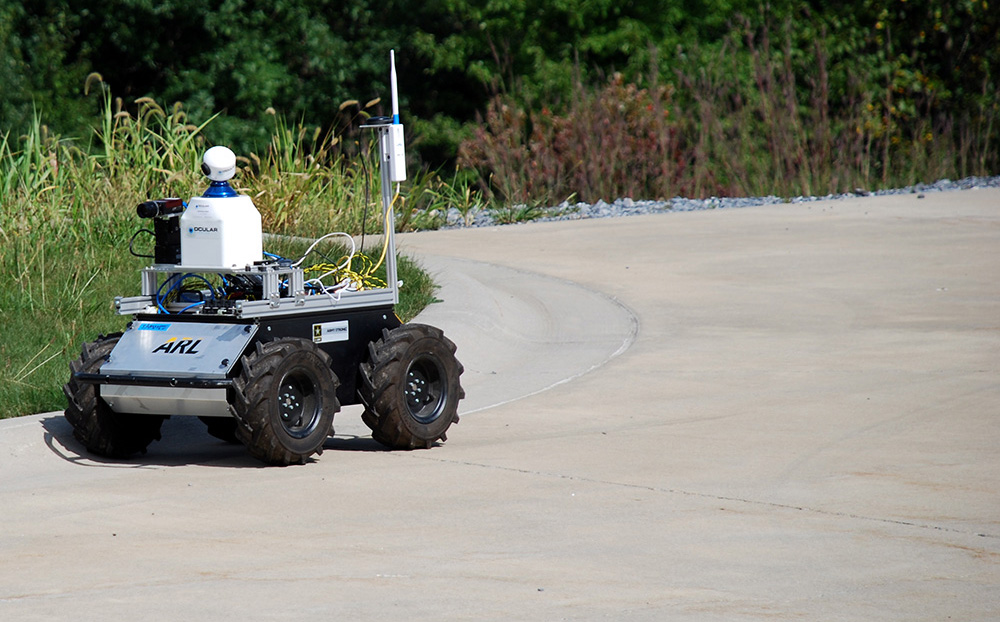
\includegraphics[width=\paperwidth]{pic1.jpg}}
\begin{frame}[t]\color{orange}\Huge{Localização na Robótica}

\end{frame}
}
%%%%%%%%%%%%%%%%%%%%%%% new slide %%%%%%%%%%%%%%%%%%%%%%%%%%%%


\begin{frame}[t]{Localização em ambientes externos}

    Em \textbf{ambientes externos}, a localização por \textbf{GPS} nem sempre oferece resultados adequados devido a \textbf{obstáculos}.
    \begin{figure}

        %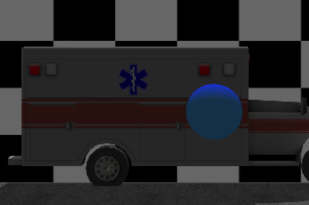
\includegraphics[width=11cm,height=6.0cm]{tf1.png}
        %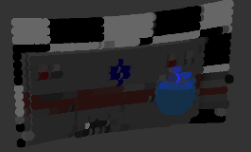
\includegraphics[width=11cm,height=6.0cm]{tf2.png}
        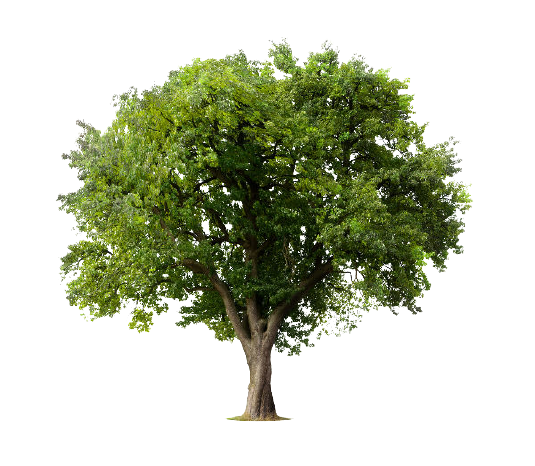
\includegraphics[width=0.475\textwidth,height=4.05cm]{pic2.png}%
        \hfill
        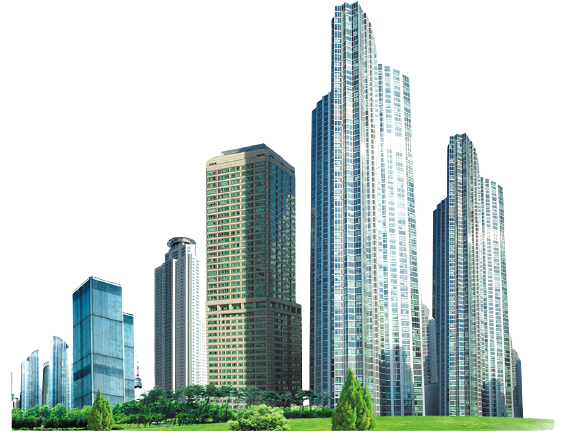
\includegraphics[width=0.475\textwidth]{pic3.png}
    
    \end{figure}

\end{frame}

%%%%%%%%%%%%%%%%%%%%%%% new slide %%%%%%%%%%%%%%%%%%%%%%%%%%%%

\begin{frame}[t]{E Agora?}

   A aplicação de \textbf{modelos probabilístico} com auxílio de \textbf{mapas} pode ser um caminho para vencer o problema de localização na robótica móvel.
   \begin{figure}
    \vspace*{0.5cm}
    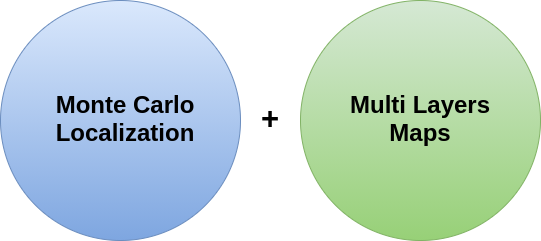
\includegraphics[width=0.4\textwidth,height=0.2\textwidth]{slide4.png}%
   \end{figure}




\end{frame}

%%%%%%%%%%%%%%%%%%%%%%% new slide %%%%%%%%%%%%%%%%%%%%%%%%%%%%

\begin{frame}[t]{Um pouco de Monte Carlo Localization}

    O Monte Carlo Localization é a aplicação de \textbf{Filtros de partículas} para Localização usando  \textbf{Inferência Bayesiana}.
    
    \begin{figure}
       
        \vspace*{0.2cm}
        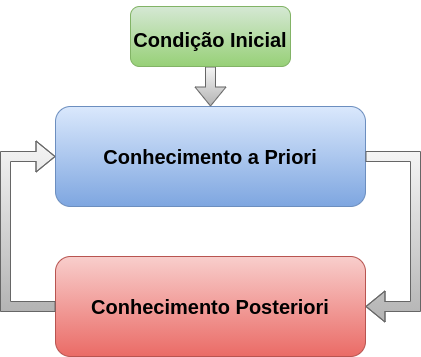
\includegraphics[width=0.435\textwidth,height=4.05cm]{inferencia.png}%
        
    
    \end{figure}
\end{frame}

%%%%%%%%%%%%%%%%%%%%%%% new slide %%%%%%%%%%%%%%%%%%%%%%%%%%%%

\begin{frame}[t]{Um pouco mais de Monte Carlo Localization}

    No \textbf{conhecimento a priori} é considerado  a \textbf{modelagem} do sistema e \textbf{conhecimento atual}. 
    \begin{figure}
        \vskip1.2cm
        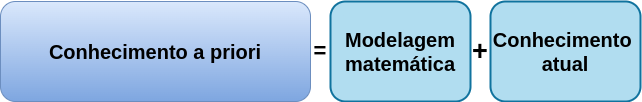
\includegraphics[width=0.635\textwidth,height=2.05cm]{priori.png}%
        
    
    \end{figure}
\end{frame}

%%%%%%%%%%%%%%%%%%%%%%% new slide %%%%%%%%%%%%%%%%%%%%%%%%%%%%

\begin{frame}[t]{Um pouco mais de Monte Carlo Localization}

    No \textbf{conhecimento a posteriori} é considerado  os \textbf{dados dos sensores} do sistema e  o\textbf{conhecimento a priori}. 
    \begin{figure}
        \vskip1.2cm
        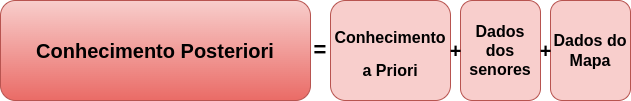
\includegraphics[width=0.635\textwidth,height=2.05cm]{posteriori.png}%
        
    
    \end{figure}
\end{frame}

%%%%%%%%%%%%%%%%%%%%%%% new slide %%%%%%%%%%%%%%%%%%%%%%%%%%%%

%\begin{frame}[c]{} 
%    \transdissolve[duration=0.5]
%   
%    \begin{center}
%        \Wider{%
%        \begin{shaded}
%        \begin{center}
%            \vspace*{0.5cm}
%            \resizebox{!}{0.7cm}{%
%                Isso é um Filtro de Kalman?
%            }%
%        \end{center}
%        \end{shaded}
%        }%
%    \end{center}
%    
%   
%%
%\end{frame}


%%%%%%%%%%%%%%%%%%%%%%% new slide %%%%%%%%%%%%%%%%%%%%%%%%%%%%

%\begin{frame}[c]{} 
%    \transdissolve[duration=0.5]
%   
%    \begin{center}
%        \Wider{%
%        \begin{shaded}
%        \begin{center}
%            \vspace*{0.5cm}
%            \resizebox{!}{0.7cm}{%
%                por um detalhe, não!
%            }%
%        \end{center}
%        \end{shaded}
%        }%
%    \end{center}
%    
%   
%%
%\end{frame}


%%%%%%%%%%%%%%%%%%%%%%% new slide %%%%%%%%%%%%%%%%%%%%%%%%%%%%



%\begin{frame}[t]{O Detalhe}
%
%    Os Filtros de Kalman são projetados sobre uma \textbf{distribuição Gaussiana}.
%    \begin{columns}[T]
%        \begin{column}{0.50\textwidth}
%            \vskip0.4cm
%            \begin{itemize}
%                \item Unimodal
%                \item Média
%                \item Variância
%                
%            \end{itemize}
%        \end{column}
%        \begin{column}{0.50\textwidth}
%            \vskip0.4cm
%            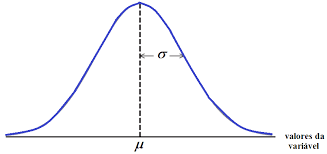
\includegraphics[width=0.735\textwidth,height=4.05cm]{gaus.png}
%            
%        \end{column}
%    \end{columns}
%   
%    
%\end{frame}

%%%%%%%%%%%%%%%%%%%%%%% new slide %%%%%%%%%%%%%%%%%%%%%%%%%%%%

\begin{frame}[t]{Ai vem as partículas}

    As \textbf{partículas} representação os \textbf{dados} que serão tratados. 
    \begin{figure}

        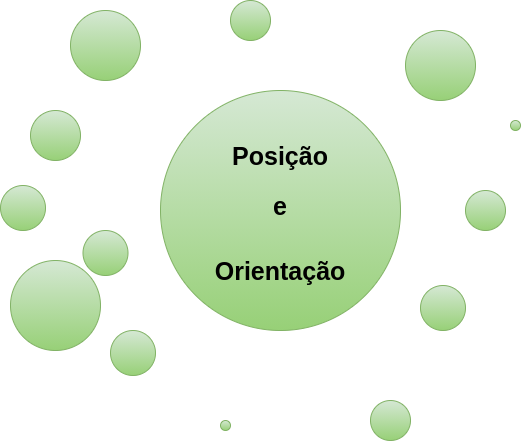
\includegraphics[width=0.610\textwidth,height=5.8cm]{particulas.png}%
        
    
    \end{figure}
\end{frame}

%%%%%%%%%%%%%%%%%%%%%%% new slide %%%%%%%%%%%%%%%%%%%%%%%%%%%%

\begin{frame}[t]{Em resumo...}

    
    \begin{figure}

        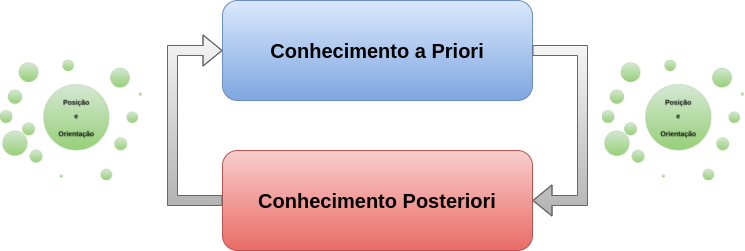
\includegraphics[width=0.830\textwidth,height=4.8cm]{mcl_resume.png}%
        
    
    \end{figure}
\end{frame}

%%%%%%%%%%%%%%%%%%%%%%% new slide %%%%%%%%%%%%%%%%%%%%%%%%%%%%

\begin{frame}[t]{Multi Layers Maps}

    \textbf{Multi Layers Maps} podem representar elevações \textbf{diferentes niveis}
    \vskip0.25cm
    \begin{figure}

        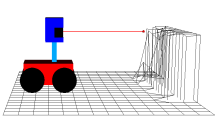
\includegraphics[width=0.630\textwidth,height=4.8cm]{mls1.png}%
        
    
    \end{figure}
\end{frame}

%%%%%%%%%%%%%%%%%%%%%%% new slide %%%%%%%%%%%%%%%%%%%%%%%%%%%%

\begin{frame}[t]{Multi Layers Maps versus Elevation maps}

    \textbf{Elevation Maps} representam as elevações usando a \textbf{média} destas.
    
    \begin{figure}

        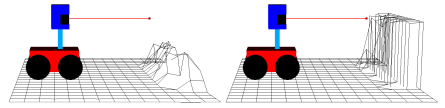
\includegraphics[width=0.630\textwidth,height=4.8cm]{mls_vs_em.png}%
        
    
    \end{figure}
\end{frame}


\begin{frame}[t]{Elevation Maps Versus Multi Layers Maps}

  
    
    \begin{figure}
        %\caption{Elevation Maps Versus Multi Layrers Maps}
        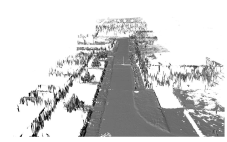
\includegraphics[width=5cm,height=5cm]{elevation.png}
        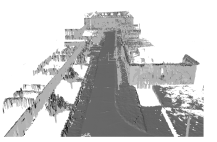
\includegraphics[width=5cm,height=5cm]{multi_layer.png}
        \label{label_here} 
    \end{figure}


    %\begin{figure}
    %    \centering
    %    \begin{subfigure}
    %      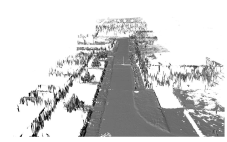
\includegraphics[width=5cm,height=5cm]{elevation.png}
    %      \caption{A subfigure}
    %      \end{subfigure}%
    %    \hfill
    %    \begin{subfigure}{}
    %     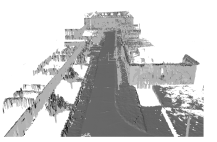
\includegraphics[width=5cm,height=5cm]{multi_layer.png}
    %      \caption{A subfigure}
    %      \end{subfigure}
    %    \caption{A figure with two subfigures}
    %\end{figure}

    
\end{frame}

%%%%%%%%%%%%%%%%%%%%%%% new slide %%%%%%%%%%%%%%%%%%%%%%%%%%%%


\begin{frame}[t]{Mais detalhes do Multi Layers Maps}

    %\textbf{Elevetion Maps} representam as elevações usando a \textbf{média} destas.
    
    \begin{itemize}
        \item São dívidas em \textbf{células quadráticas}.
        \item Cada célula possui um \textbf{vetor normal} com a superfície
        \item É capaz de detectar \textbf{pontes e passagens elevadas}.
        \item Os dados \textbf{verticais} podem ser usados para \textbf{estimar a posição} do robô.
        \item O \textbf{custo computacional} é de apenas \textbf{10\% maior}. 
     
    \end{itemize}

\end{frame}

%%%%%%%%%%%%%%%%%%%%%%% new slide %%%%%%%%%%%%%%%%%%%%%%%%%%%%

\begin{frame}[c]{Monte Carlo com Multi Layers Maps} 
    \transdissolve[duration=0.5]
   
    \begin{center}
        \Wider{%
        \begin{shaded}
        \begin{center}
            \vspace*{0.5cm}
            \resizebox{!}{0.7cm}{%
                Predição
            }%
        \end{center}
        \end{shaded}
        }%
    \end{center}
    
   
%
\end{frame}

%%%%%%%%%%%%%%%%%%%%%%% new slide %%%%%%%%%%%%%%%%%%%%%%%%%%%%

\begin{frame}[t]{Predição}
    O \textbf{Modelo Probabilístico} trata os \textbf{vetores de movimentos em 2D}, mas  o \textbf{MLS} é necessário uma transformação em 3D.
    %\textbf{Elevetion Maps} representam as elevações usando a \textbf{média} destas.
    
    \begin{figure}

        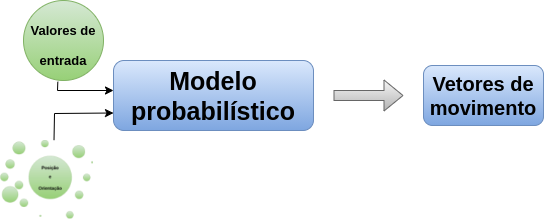
\includegraphics[width=0.730\textwidth,height=4.8cm]{pred1.png}%
        
    
    \end{figure}
\end{frame}

%%%%%%%%%%%%%%%%%%%%%%% new slide %%%%%%%%%%%%%%%%%%%%%%%%%%%%

\begin{frame}[t]{Predição com auxilio do Mapa}
    Considerando a existência de \textbf{vetores normais} a superfície para célula, é possivél tranformar um \textbf{vetor de movimento 2D}  em \textbf{3D}.
    %\textbf{Elevetion Maps} representam as elevações usando a \textbf{média} destas.
    
    \begin{figure}

        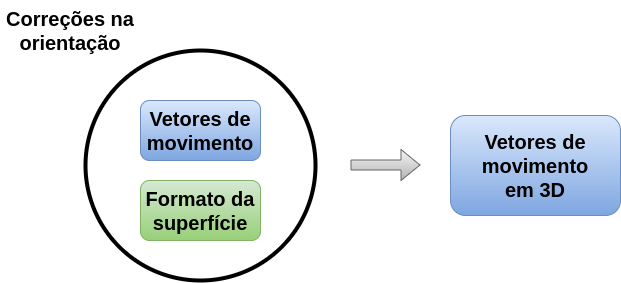
\includegraphics[width=0.730\textwidth,height=4.8cm]{pred2.png}%
        
    
    \end{figure}
\end{frame}

%%%%%%%%%%%%%%%%%%%%%%% new slide %%%%%%%%%%%%%%%%%%%%%%%%%%%%

%\begin{frame}[t]{Predição com auxilio do Mapa}
%    .
%    %\textbf{Elevetion Maps} representam as elevações usando a \textbf{média} destas.
%    
%    \begin{figure}
%
%        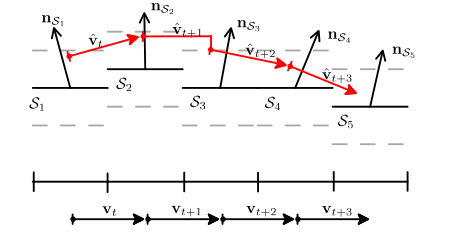
\includegraphics[width=0.630\textwidth,height=4.8cm]{pp2.png}%
%        
%    
%    \end{figure}
%\end{frame}

%%%%%%%%%%%%%%%%%%%%%%% new slide %%%%%%%%%%%%%%%%%%%%%%%%%%%%

\begin{frame}[c]{Monte Carlo com Multi Layers Maps} 
    \transdissolve[duration=0.5]
   
    \begin{center}
        \Wider{%
        \begin{shaded}
        \begin{center}
            \vspace*{0.5cm}
            \resizebox{!}{0.7cm}{%
                Modelo Sensorial para MLS
            }%
        \end{center}
        \end{shaded}
        }%
    \end{center}
    
   
%
\end{frame}

%%%%%%%%%%%%%%%%%%%%%%% new slide %%%%%%%%%%%%%%%%%%%%%%%%%%%%

\begin{frame}[c]{} 
    \transdissolve[duration=0.5]
   
    \begin{center}
        \Wider{%
        \begin{shaded}
        \begin{center}
            \vspace*{0.5cm}
            \resizebox{!}{0.7cm}{%
                Resultados
            }%
        \end{center}
        \end{shaded}
        }%
    \end{center}
    
   
%
\end{frame}

%%%%%%%%%%%%%%%%%%%%%%% new slide %%%%%%%%%%%%%%%%%%%%%%%%%%%%




\begin{frame}[t]{Elevation Maps Vs Multi Layers Superficies}
    
    %\textbf{Elevetion Maps} representam as elevações usando a \textbf{média} destas.
    
    \begin{figure}

        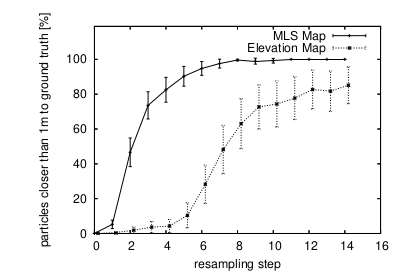
\includegraphics[width=0.730\textwidth,height=5.1cm]{results1.png}%
        
    
    \end{figure}
\end{frame}

%%%%%%%%%%%%%%%%%%%%%%% new slide %%%%%%%%%%%%%%%%%%%%%%%%%%%%
\begin{frame}[t]{Mapa Conceitual}
 
    \begin{figure}

        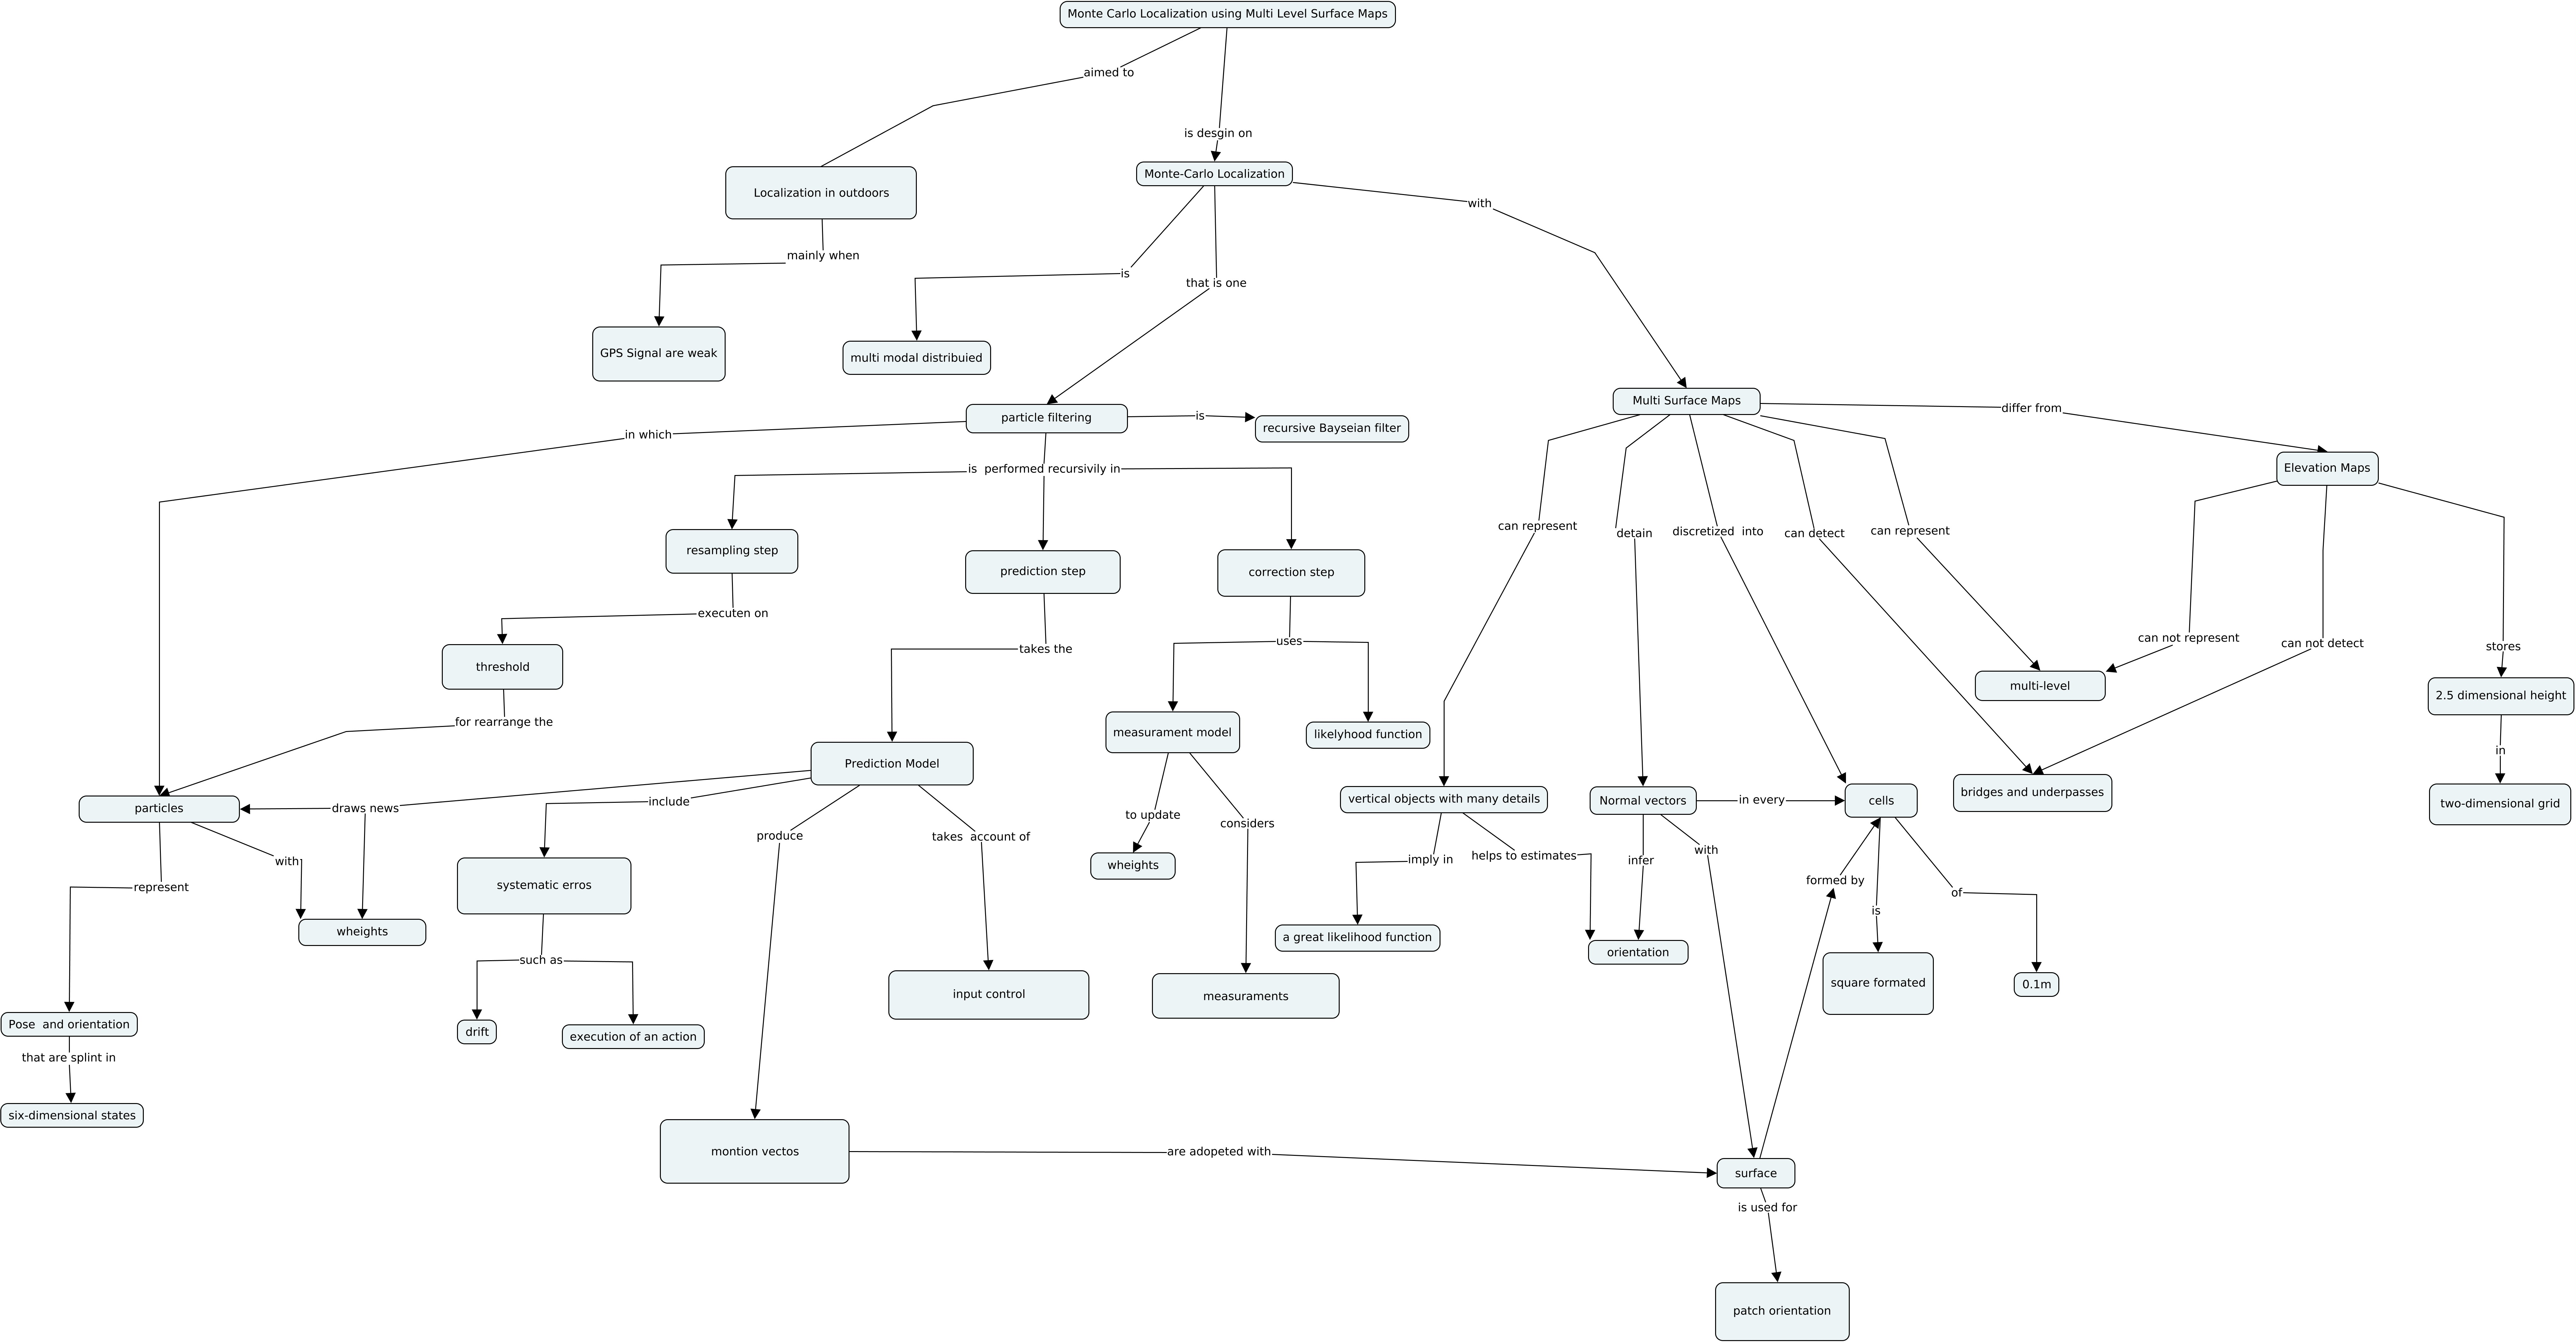
\includegraphics[width=350]{conceptual_map.jpg}%
        
    
    \end{figure}
\end{frame}
\begin{frame}[c]{} 
    \transdissolve[duration=0.5]
   
    \begin{center}
        \Wider{%
        \begin{shaded}
        \begin{center}
            \vspace*{0.5cm}
            \resizebox{!}{0.7cm}{%
            Conclusão
            }%
        \end{center}
        \end{shaded}
        }%
    \end{center}
    
   
%
\end{frame}